%proportional corrected algorithm methods
We attempted to correct the dark spot issue by significantly reducing the absolute difference between dark pixels and the average colour, ensuring that the dark spots would instead have colours close to the average. We perform this correction on the output of the proportional adjustment algorithm.

\begin{algorithm}[H]
\caption{Dark spot correction}
\label{eq:prop_corr_algo}
\begin{algorithmic}
\State Let $\alpha$ be a constant, $\alpha  > 1$. We expect that the larger the value of alpha, the stronger the effect of the reduced dark spot.
\State Let $O$ be the set of pixels in the output image, and $W \subseteq O$ be the set of pixels used to calculate the average colour of the output image. $W$ corresponds to the region $V \subseteq S$, and $\left|W\right| = \left|V\right|$ \\
\State We calculate the average skin colour of the output of Algorithm \ref{eq:prop_algo}
\State $\mean{C_O} \gets \Call{Mean}{\vect{C_O}(W)}$\\
\State For all pixels below the average colour we limit their distance to the average 
\For{each pixel $i \in O$}
\If{$\vect{C_O}(i) \leq \mean{C_O}$}
\State $\vect{C_O}(i) \gets \displaystyle \mean{C_O} - \frac{\left(\mean{C_O} - \vect{C_O}(i)\right)}{\alpha}$
\EndIf
\EndFor
\end{algorithmic}
\end{algorithm}

\nomenclature{$\mean{C_S}$}{The average RGB color of the output hand}
\nomenclature{$W$}{The subset of pixels used to calculate the average color of the hand in the output image}
\nomenclature{$\alpha$}{The constant used to determine the strength of the dark spot correction}

In Table \ref{tab:prop_correct_test_a1p1} we show the results for colour transfers between all possible combinations of our test images for $\alpha = 1.1$. The results for some of the other $\alpha$ values we tried are shown in Appendices \ref{app:prop_corr_ave_a1p5} and \ref{app:prop_corr_ave_a5}.

\begin{longtable}{|N||c|c|c|}
	\caption{Test results of proportional brightening with correction for dark spots, alpha = 1.1\label{tab:prop_correct_test_a1p1}}\\
	\hline
	\multicolumn{1}{|c||}{No.} & Original & Target & Results \\ 
	\hline
	    \label{row:prop_correct_test_a1p1_hand_dark_to_hand_brown} &
  \begin{minipage}{.29\textwidth}
    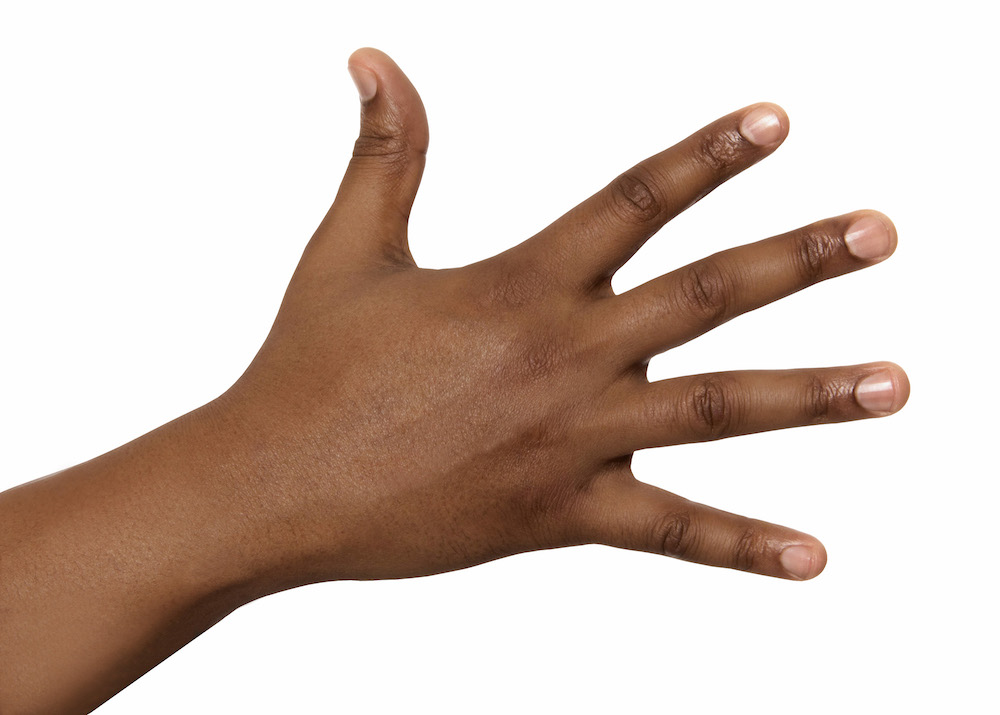
\includegraphics[width=\textwidth,height=\textheight,keepaspectratio]{../inputs/hand_dark.jpg}
  \end{minipage} & 
  \begin{minipage}{.29\textwidth}
    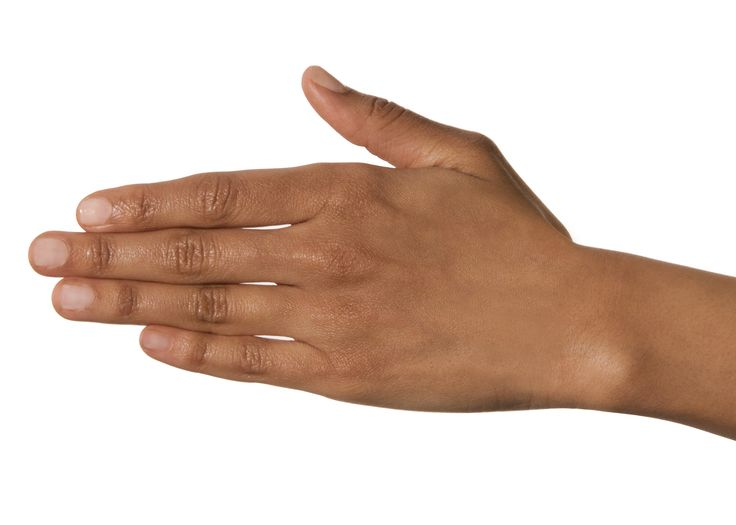
\includegraphics[width=\textwidth,height=\textheight,keepaspectratio]{../inputs/hand_brown.jpg}
  \end{minipage} & 
  \begin{minipage}{.29\textwidth}
    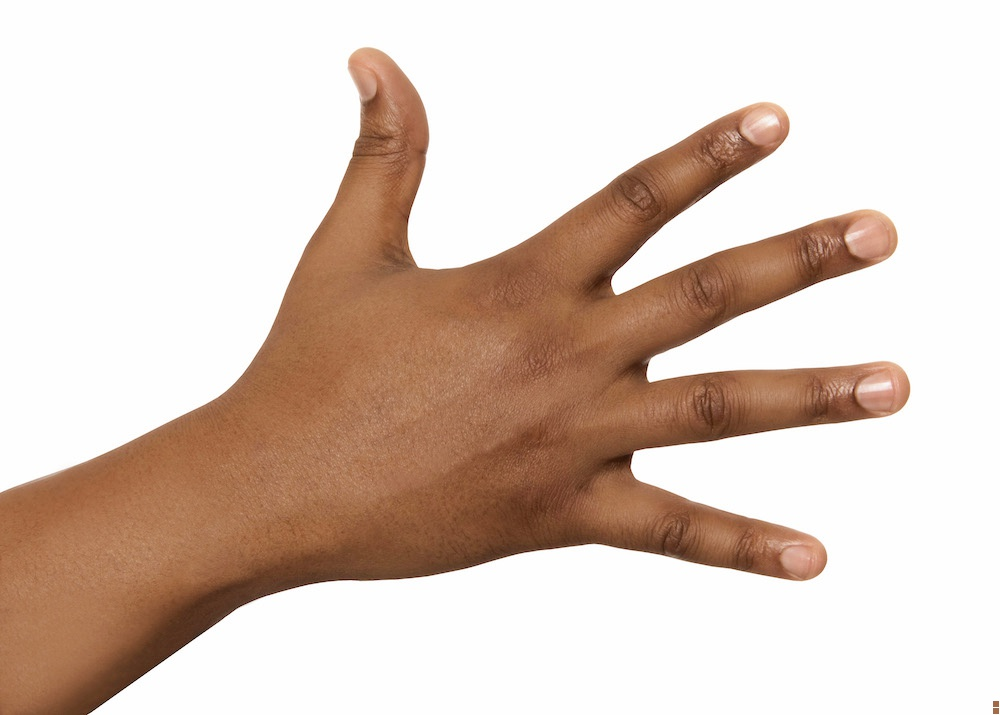
\includegraphics[width=\textwidth,height=\textheight,keepaspectratio]{../rc_test/outputs/20170522_proportional_corrected_test_alpha1p1/hand_dark_to_hand_brown.jpg}
  \end{minipage} \\
\hline  \label{row:prop_correct_test_a1p1_hand_dark_to_hand_light} &
  \begin{minipage}{.29\textwidth}
    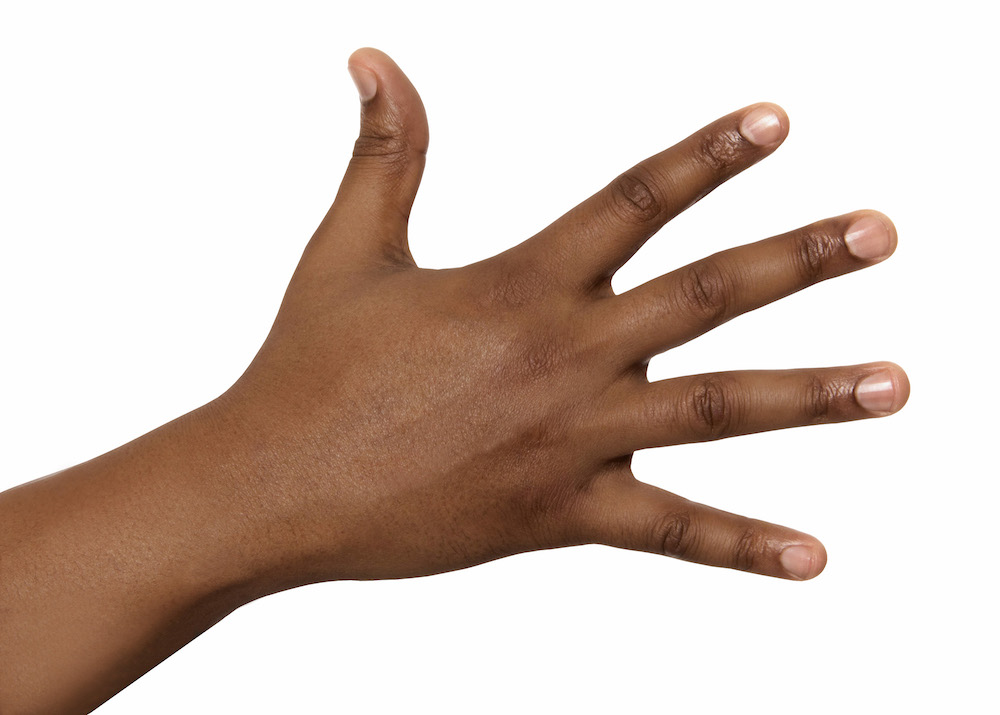
\includegraphics[width=\textwidth,height=\textheight,keepaspectratio]{../inputs/hand_dark.jpg}
  \end{minipage} & 
  \begin{minipage}{.29\textwidth}
    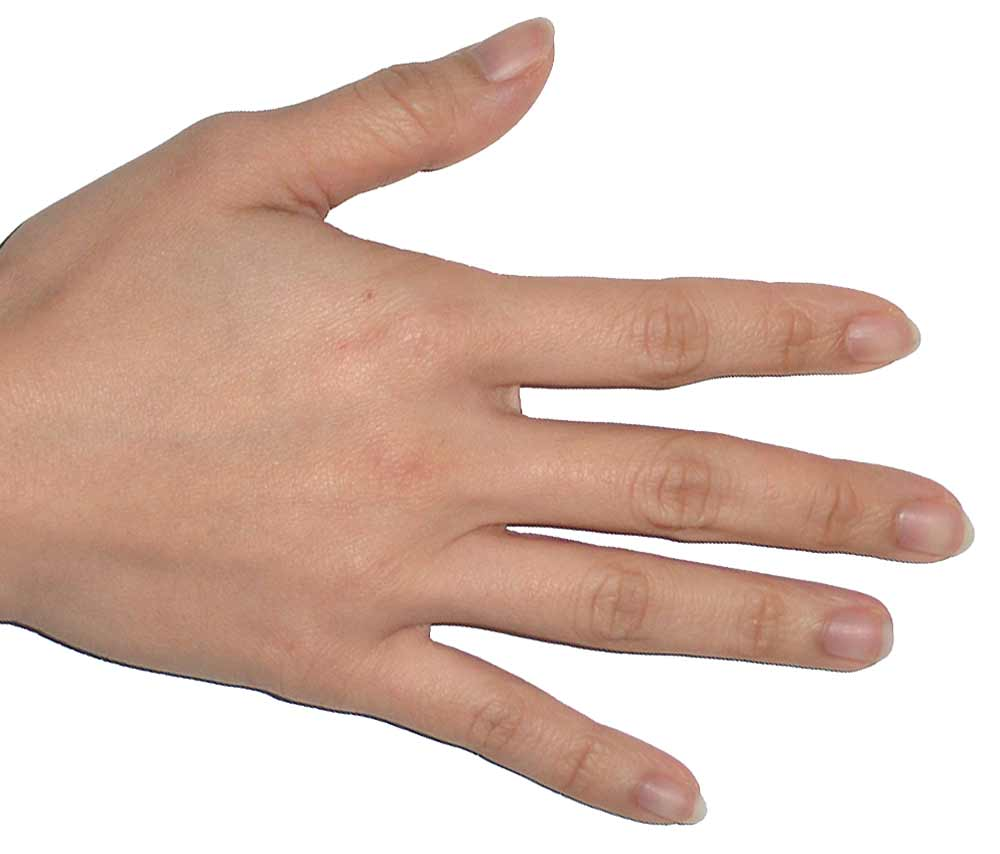
\includegraphics[width=\textwidth,height=\textheight,keepaspectratio]{../inputs/hand_light.jpg}
  \end{minipage} & 
  \begin{minipage}{.29\textwidth}
    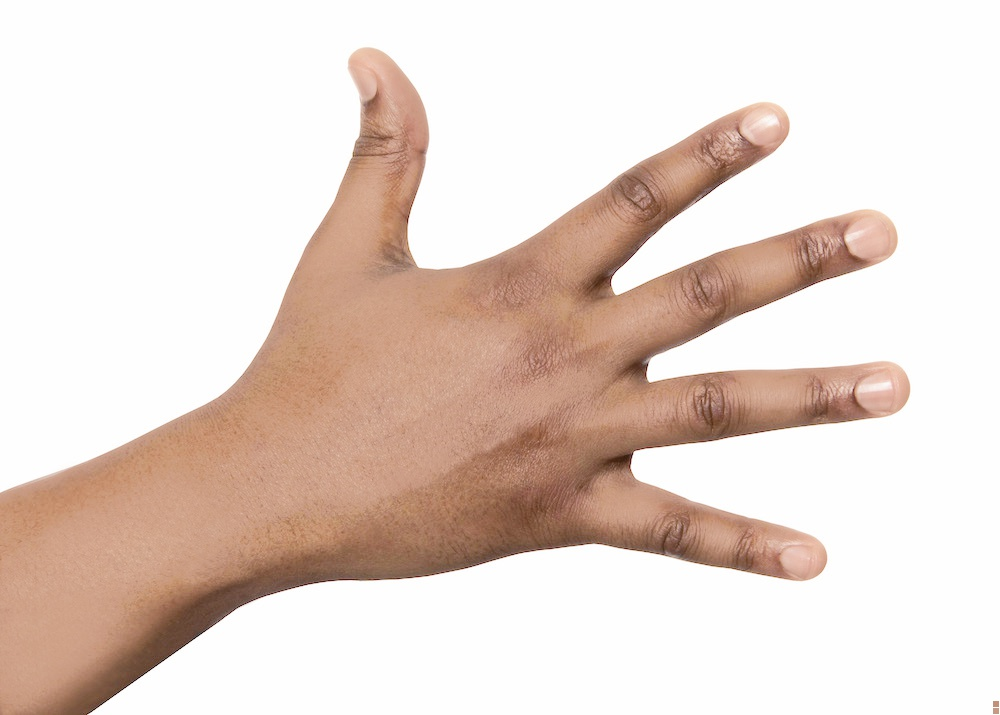
\includegraphics[width=\textwidth,height=\textheight,keepaspectratio]{../rc_test/outputs/20170522_proportional_corrected_test_alpha1p1/hand_dark_to_hand_light.jpg}
  \end{minipage} \\
\hline  \label{row:prop_correct_test_a1p1_hand_dark_to_hand_pale} &
  \begin{minipage}{.29\textwidth}
    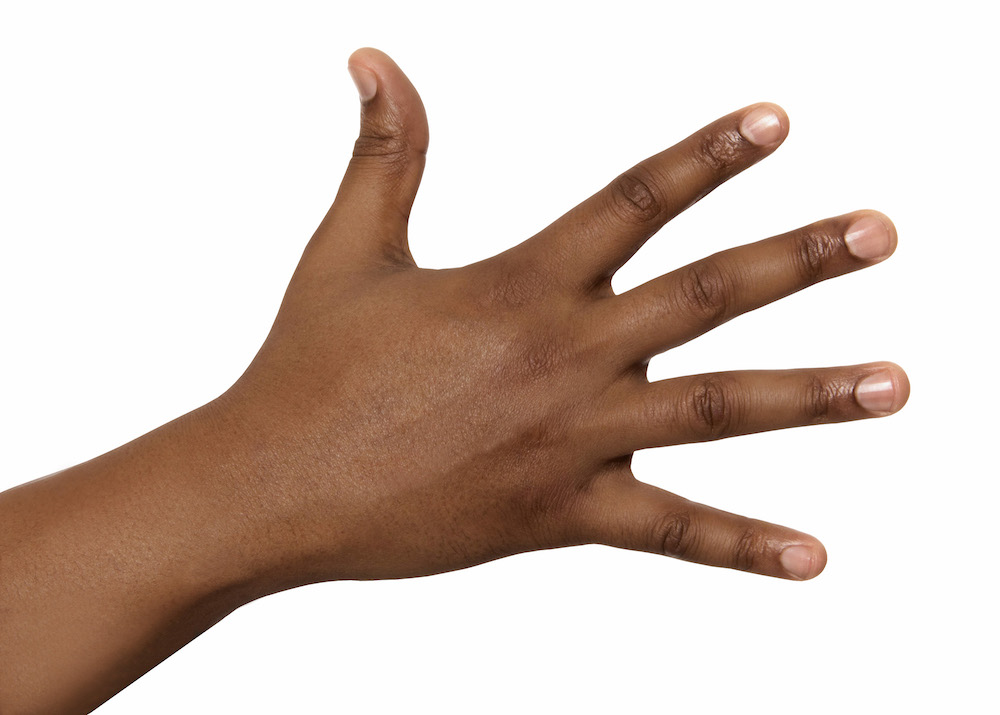
\includegraphics[width=\textwidth,height=\textheight,keepaspectratio]{../inputs/hand_dark.jpg}
  \end{minipage} & 
  \begin{minipage}{.29\textwidth}
    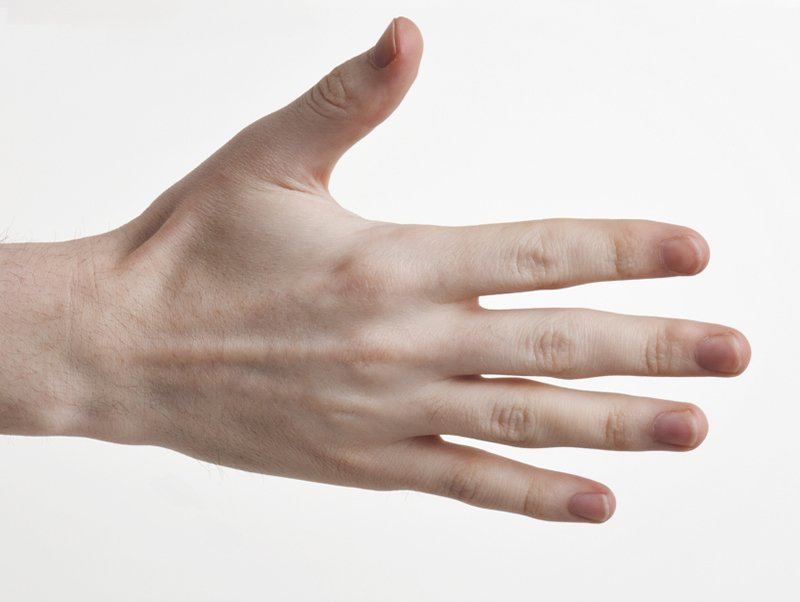
\includegraphics[width=\textwidth,height=\textheight,keepaspectratio]{../inputs/hand_pale.jpg}
  \end{minipage} & 
  \begin{minipage}{.29\textwidth}
    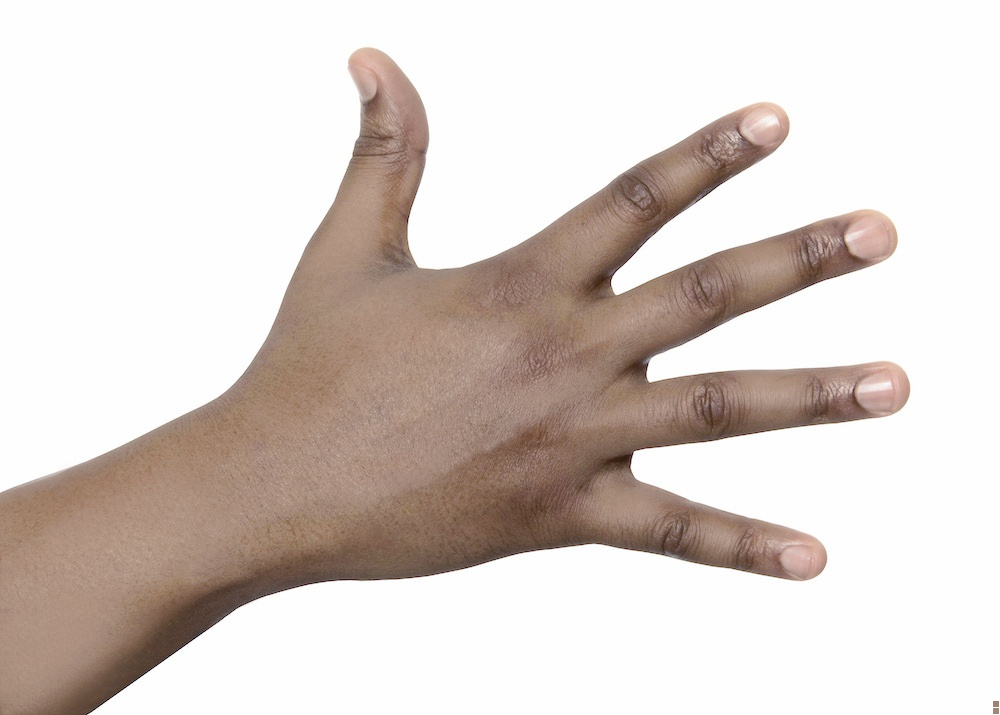
\includegraphics[width=\textwidth,height=\textheight,keepaspectratio]{../rc_test/outputs/20170522_proportional_corrected_test_alpha1p1/hand_dark_to_hand_pale.jpg}
  \end{minipage} \\
\hline  \label{row:prop_correct_test_a1p1_hand_brown_to_hand_dark} &
  \begin{minipage}{.29\textwidth}
    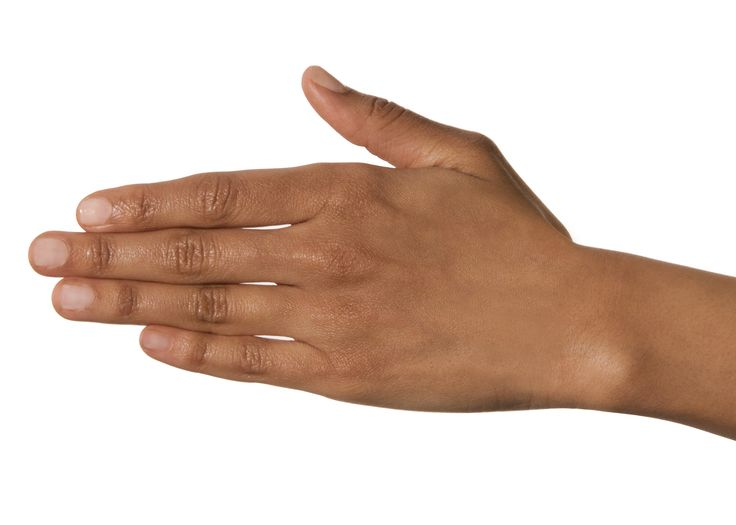
\includegraphics[width=\textwidth,height=\textheight,keepaspectratio]{../inputs/hand_brown.jpg}
  \end{minipage} & 
  \begin{minipage}{.29\textwidth}
    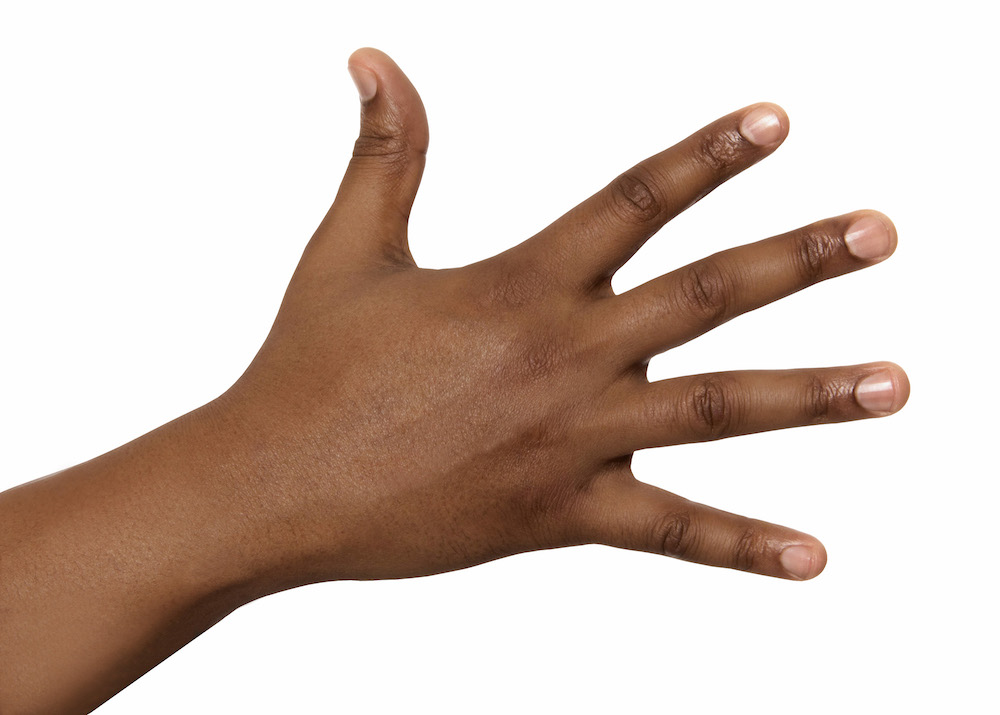
\includegraphics[width=\textwidth,height=\textheight,keepaspectratio]{../inputs/hand_dark.jpg}
  \end{minipage} & 
  \begin{minipage}{.29\textwidth}
    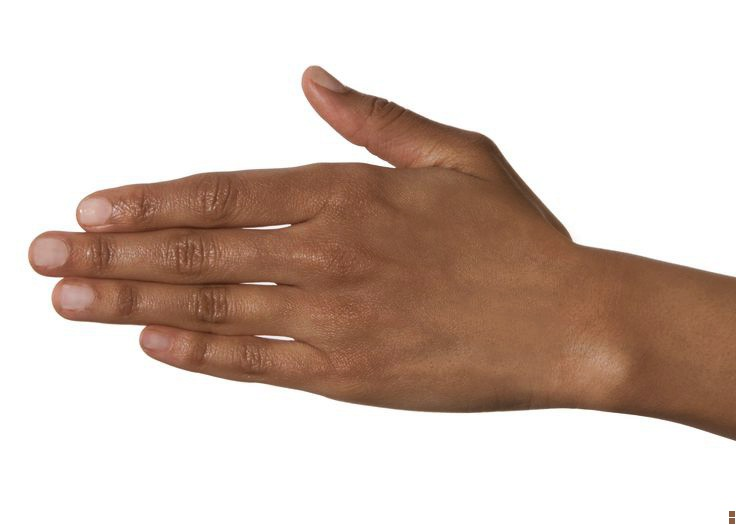
\includegraphics[width=\textwidth,height=\textheight,keepaspectratio]{../rc_test/outputs/20170522_proportional_corrected_test_alpha1p1/hand_brown_to_hand_dark.jpg}
  \end{minipage} \\
\hline  \label{row:prop_correct_test_a1p1_hand_brown_to_hand_light} &
  \begin{minipage}{.29\textwidth}
    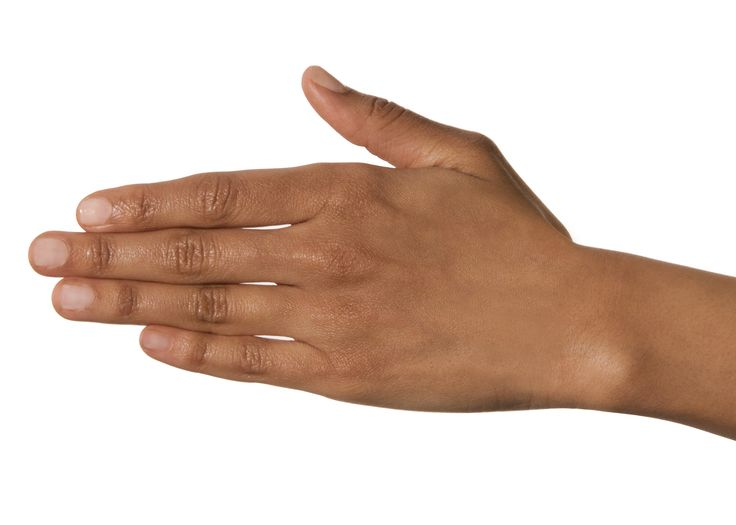
\includegraphics[width=\textwidth,height=\textheight,keepaspectratio]{../inputs/hand_brown.jpg}
  \end{minipage} & 
  \begin{minipage}{.29\textwidth}
    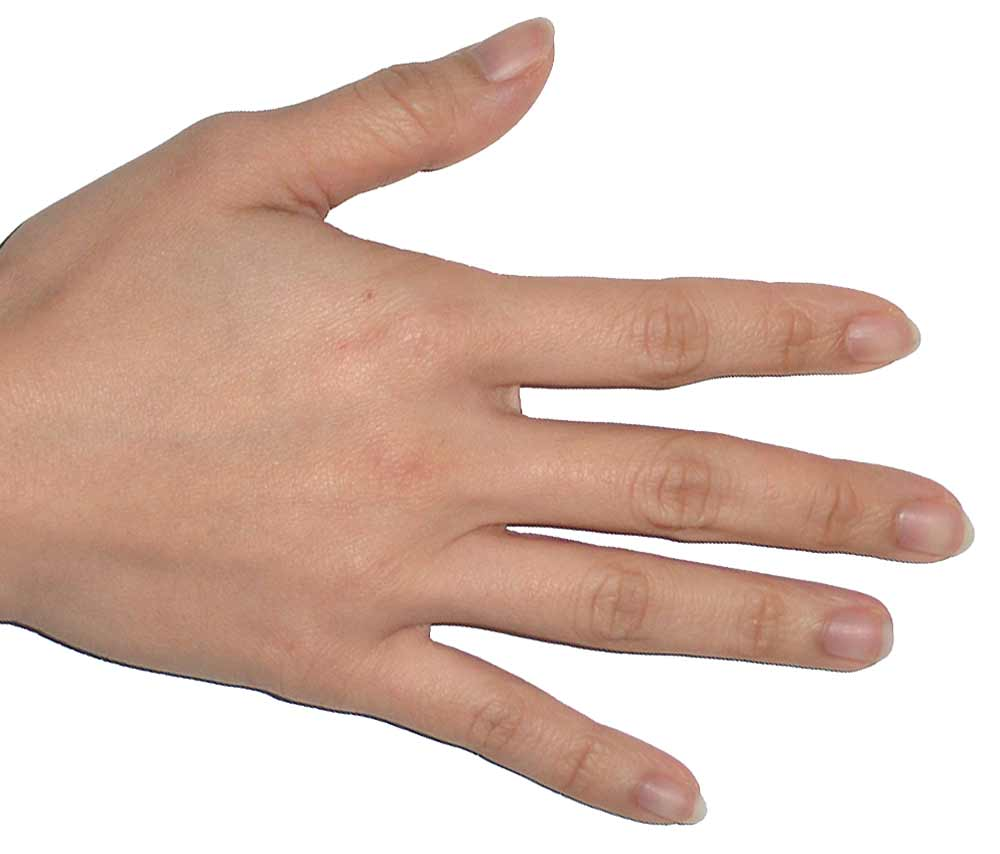
\includegraphics[width=\textwidth,height=\textheight,keepaspectratio]{../inputs/hand_light.jpg}
  \end{minipage} & 
  \begin{minipage}{.29\textwidth}
    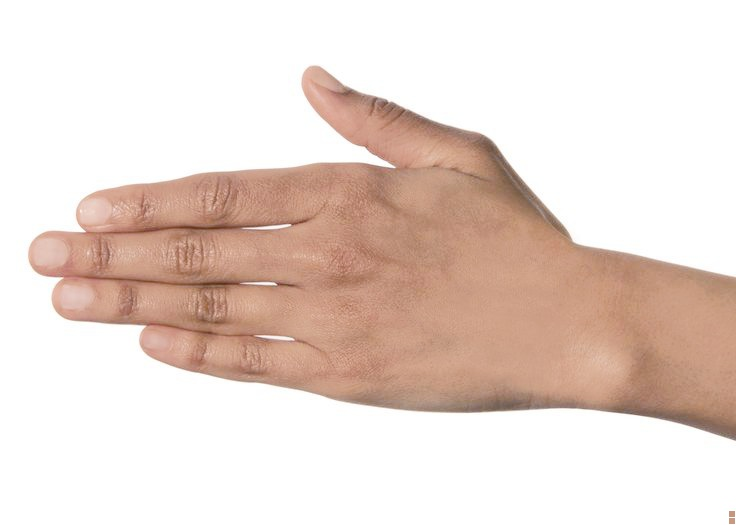
\includegraphics[width=\textwidth,height=\textheight,keepaspectratio]{../rc_test/outputs/20170522_proportional_corrected_test_alpha1p1/hand_brown_to_hand_light.jpg}
  \end{minipage} \\
\hline  \label{row:prop_correct_test_a1p1_hand_brown_to_hand_pale} &
  \begin{minipage}{.29\textwidth}
    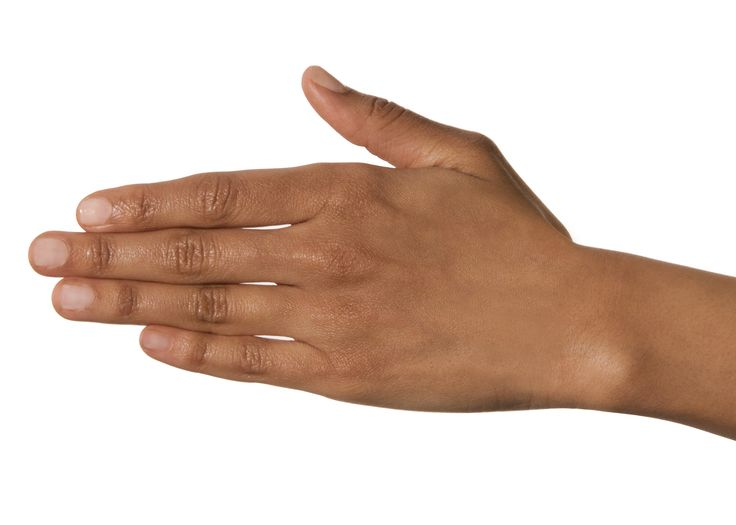
\includegraphics[width=\textwidth,height=\textheight,keepaspectratio]{../inputs/hand_brown.jpg}
  \end{minipage} & 
  \begin{minipage}{.29\textwidth}
    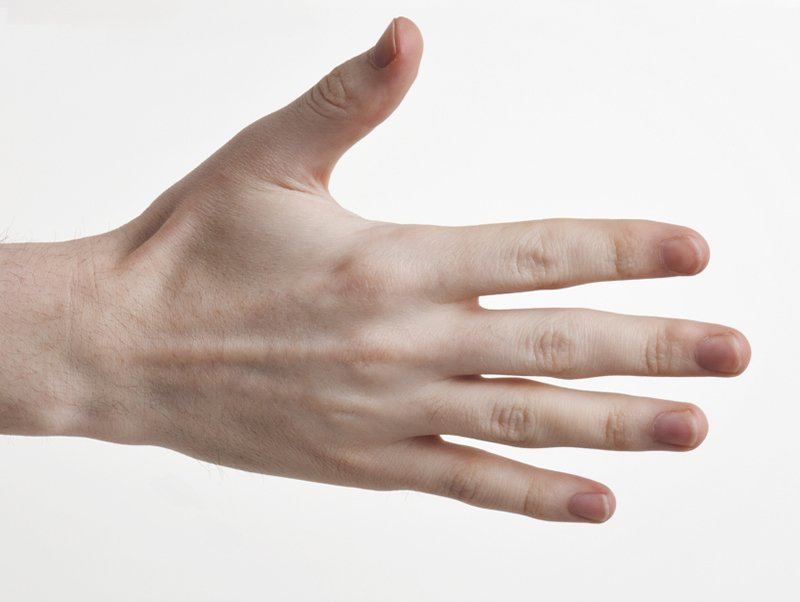
\includegraphics[width=\textwidth,height=\textheight,keepaspectratio]{../inputs/hand_pale.jpg}
  \end{minipage} & 
  \begin{minipage}{.29\textwidth}
    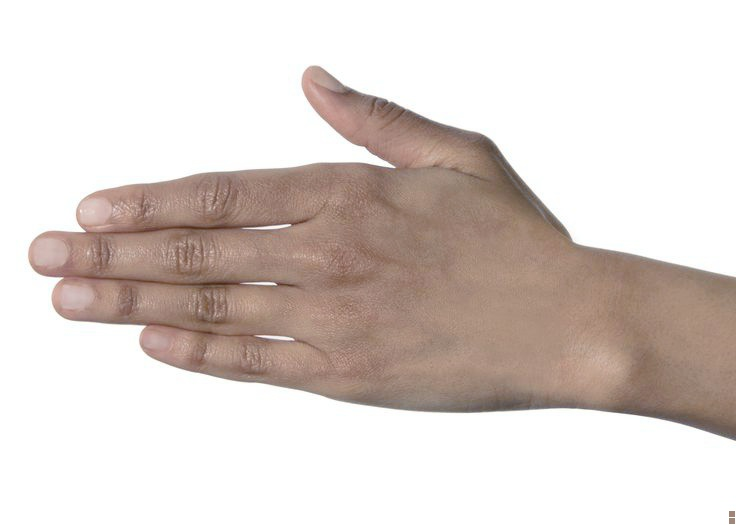
\includegraphics[width=\textwidth,height=\textheight,keepaspectratio]{../rc_test/outputs/20170522_proportional_corrected_test_alpha1p1/hand_brown_to_hand_pale.jpg}
  \end{minipage} \\
\hline  \label{row:prop_correct_test_a1p1_hand_light_to_hand_dark} &
  \begin{minipage}{.29\textwidth}
    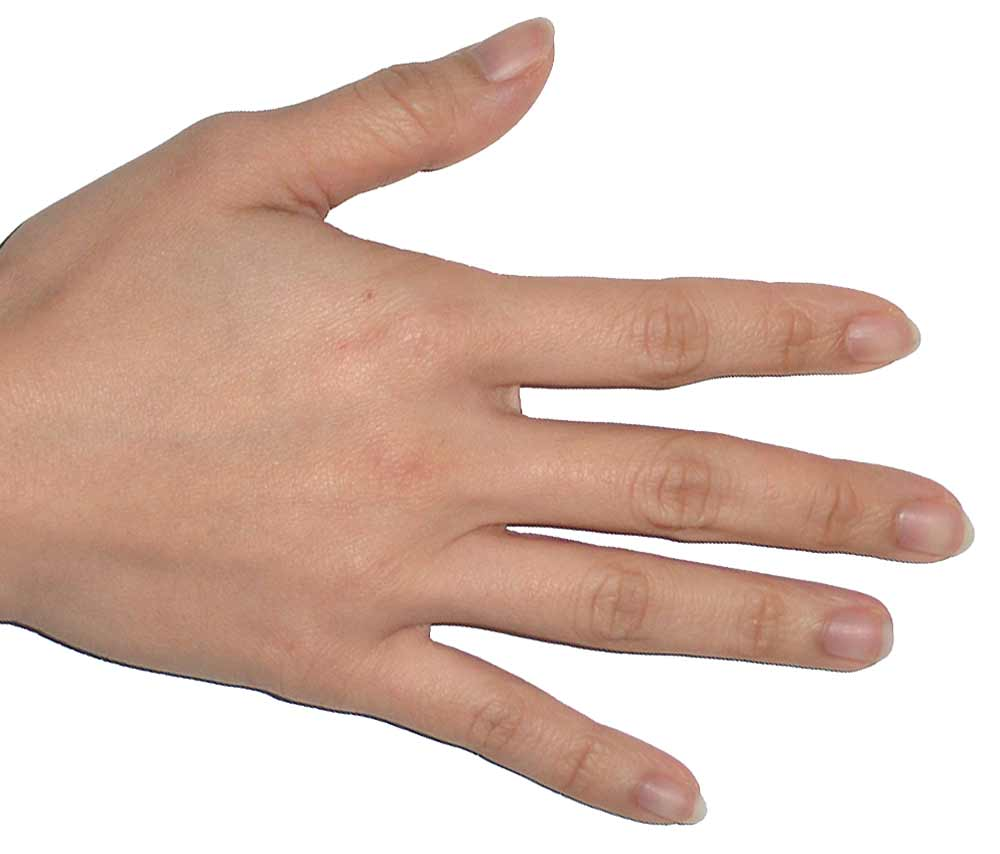
\includegraphics[width=\textwidth,height=\textheight,keepaspectratio]{../inputs/hand_light.jpg}
  \end{minipage} & 
  \begin{minipage}{.29\textwidth}
    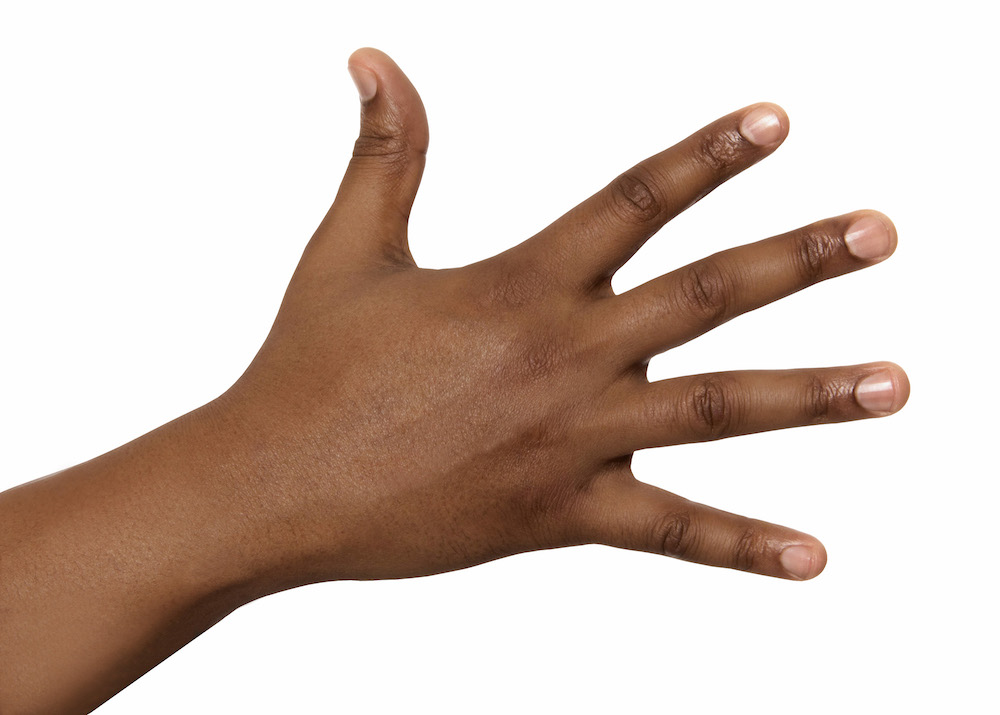
\includegraphics[width=\textwidth,height=\textheight,keepaspectratio]{../inputs/hand_dark.jpg}
  \end{minipage} & 
  \begin{minipage}{.29\textwidth}
    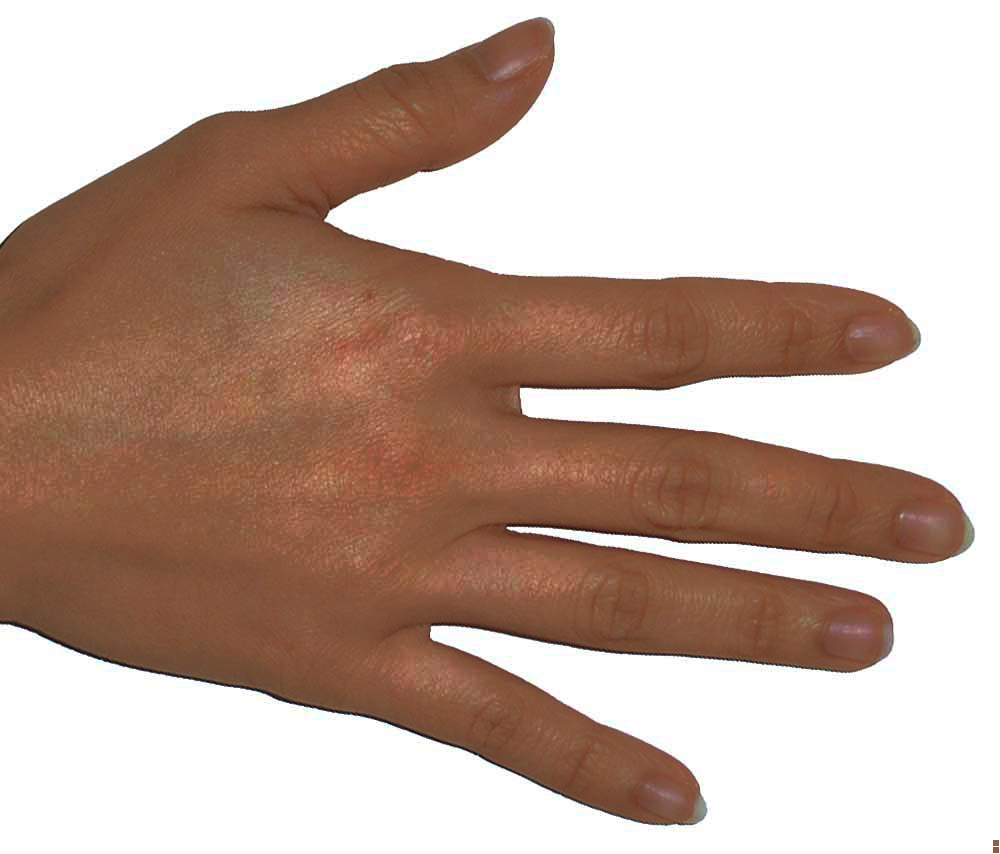
\includegraphics[width=\textwidth,height=\textheight,keepaspectratio]{../rc_test/outputs/20170522_proportional_corrected_test_alpha1p1/hand_light_to_hand_dark.jpg}
  \end{minipage} \\
\hline  \label{row:prop_correct_test_a1p1_hand_light_to_hand_brown} &
  \begin{minipage}{.29\textwidth}
    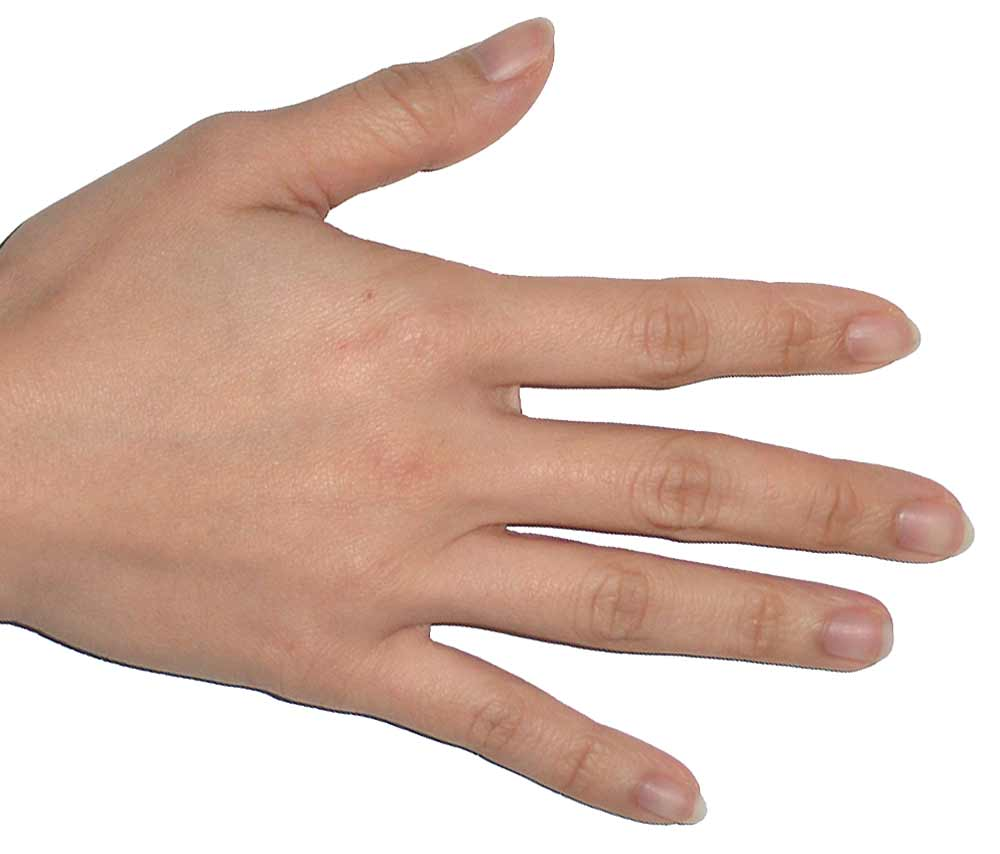
\includegraphics[width=\textwidth,height=\textheight,keepaspectratio]{../inputs/hand_light.jpg}
  \end{minipage} & 
  \begin{minipage}{.29\textwidth}
    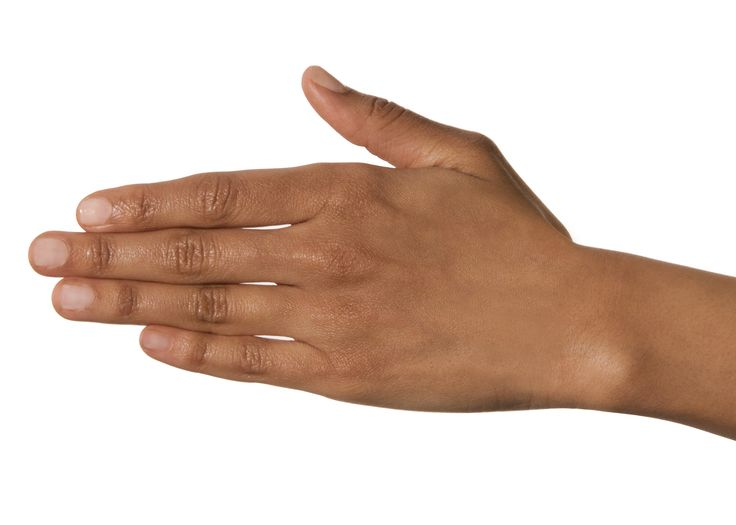
\includegraphics[width=\textwidth,height=\textheight,keepaspectratio]{../inputs/hand_brown.jpg}
  \end{minipage} & 
  \begin{minipage}{.29\textwidth}
    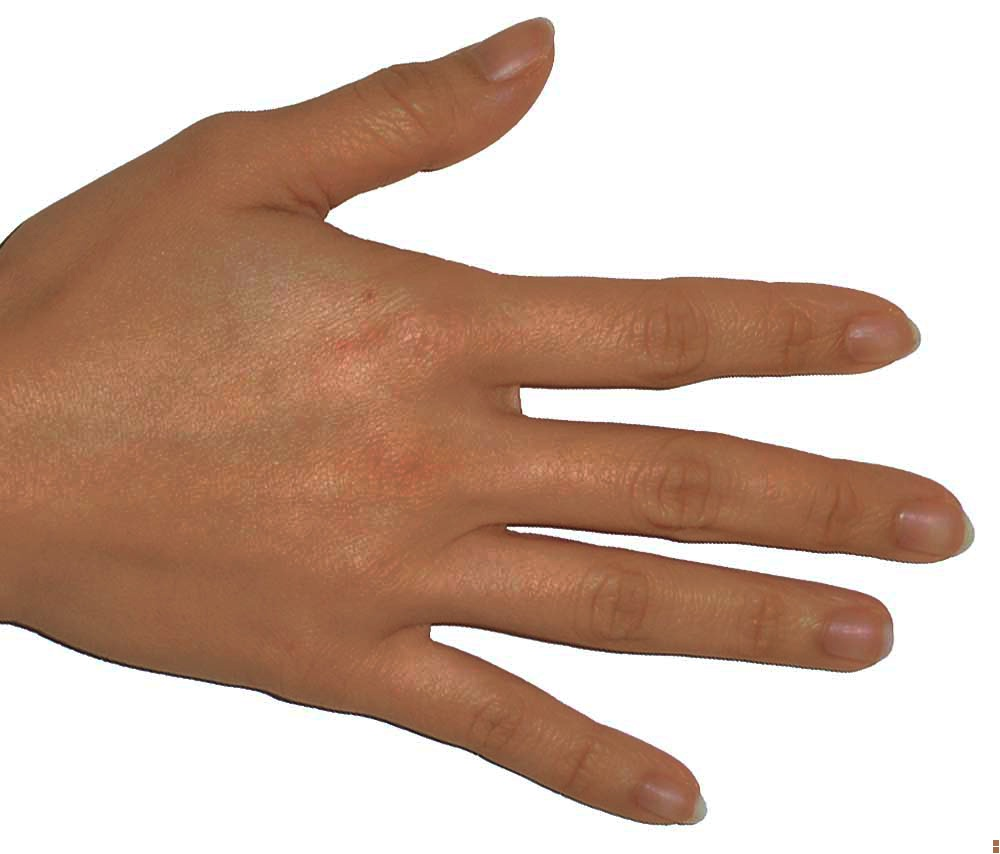
\includegraphics[width=\textwidth,height=\textheight,keepaspectratio]{../rc_test/outputs/20170522_proportional_corrected_test_alpha1p1/hand_light_to_hand_brown.jpg}
  \end{minipage} \\
\hline  \label{row:prop_correct_test_a1p1_hand_light_to_hand_pale} &
  \begin{minipage}{.29\textwidth}
    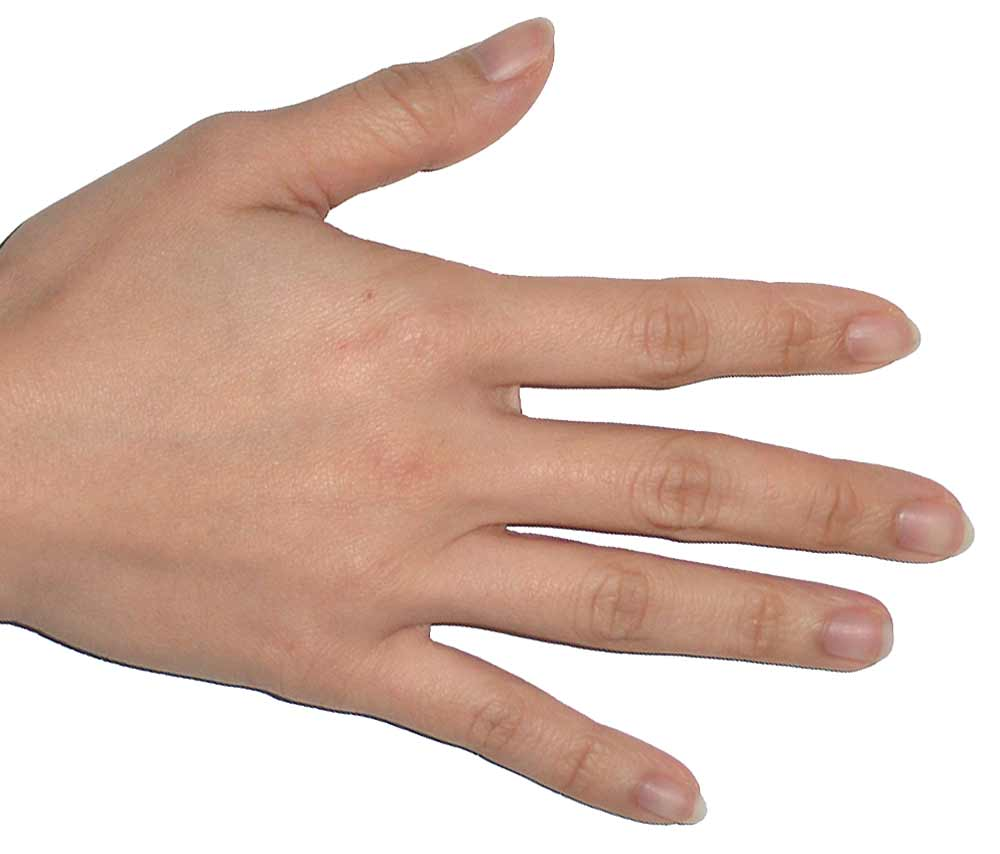
\includegraphics[width=\textwidth,height=\textheight,keepaspectratio]{../inputs/hand_light.jpg}
  \end{minipage} & 
  \begin{minipage}{.29\textwidth}
    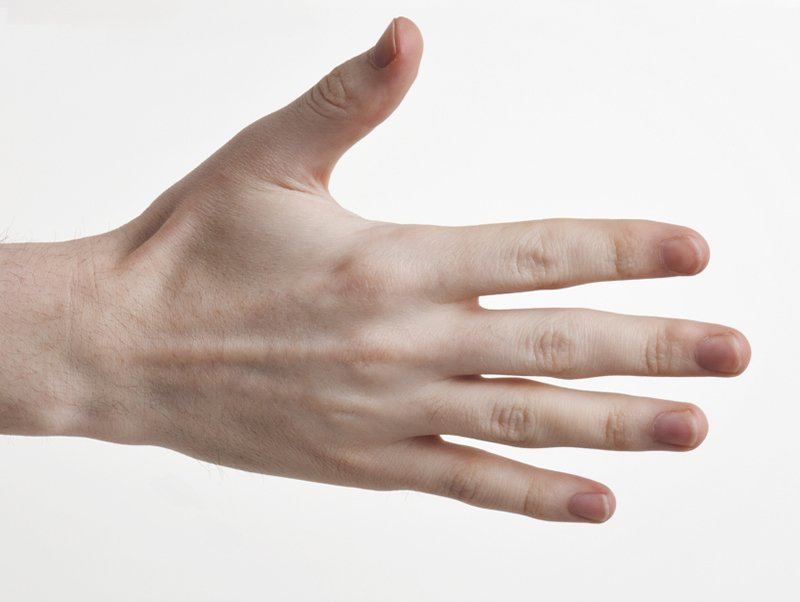
\includegraphics[width=\textwidth,height=\textheight,keepaspectratio]{../inputs/hand_pale.jpg}
  \end{minipage} & 
  \begin{minipage}{.29\textwidth}
    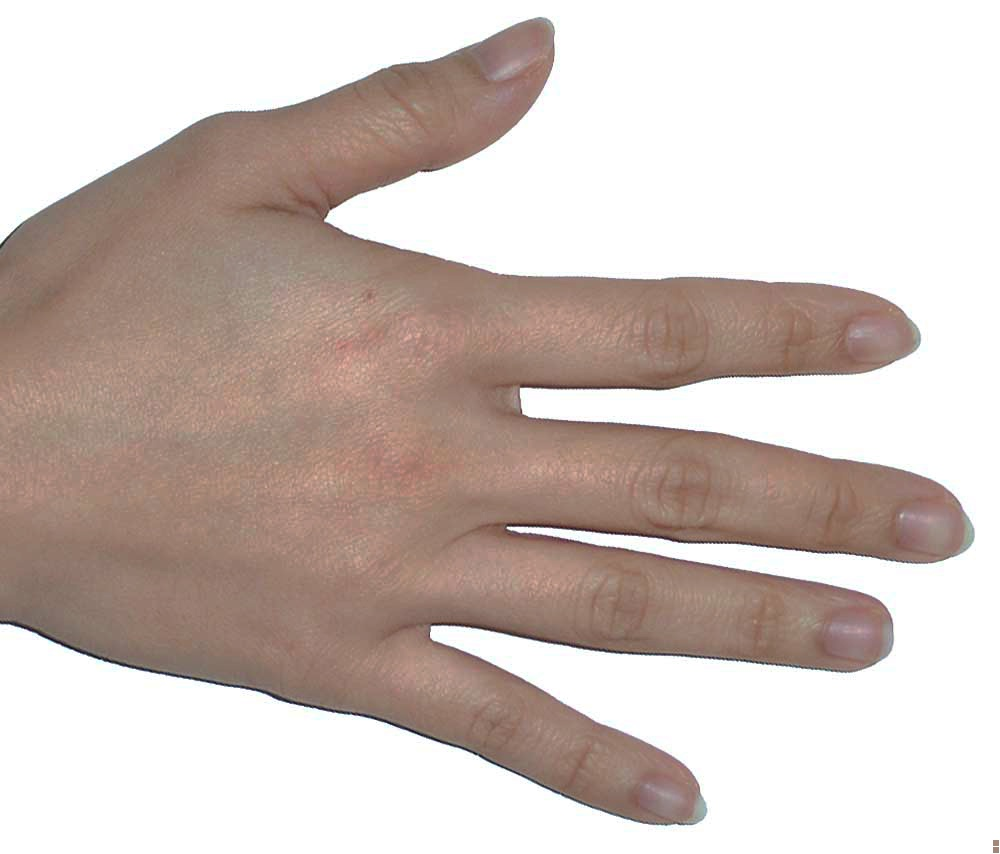
\includegraphics[width=\textwidth,height=\textheight,keepaspectratio]{../rc_test/outputs/20170522_proportional_corrected_test_alpha1p1/hand_light_to_hand_pale.jpg}
  \end{minipage} \\
\hline  \label{row:prop_correct_test_a1p1_hand_pale_to_hand_dark} &
  \begin{minipage}{.29\textwidth}
    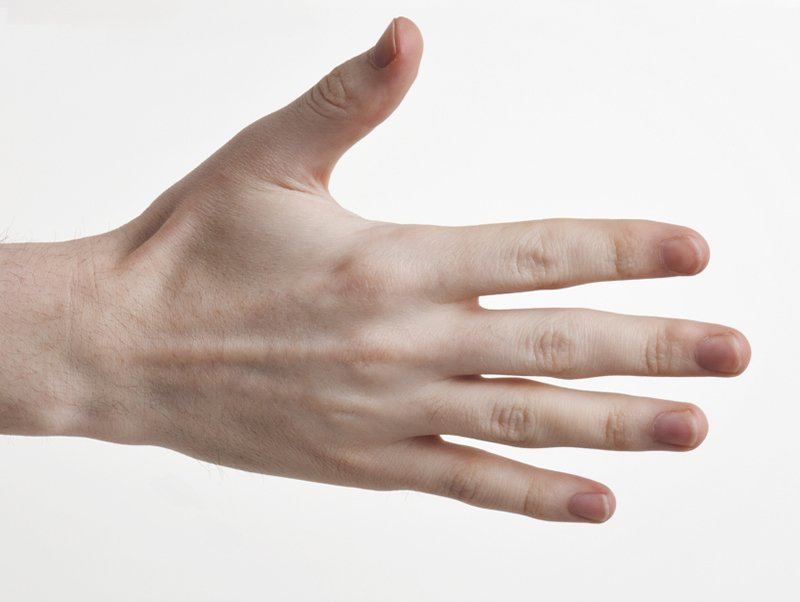
\includegraphics[width=\textwidth,height=\textheight,keepaspectratio]{../inputs/hand_pale.jpg}
  \end{minipage} & 
  \begin{minipage}{.29\textwidth}
    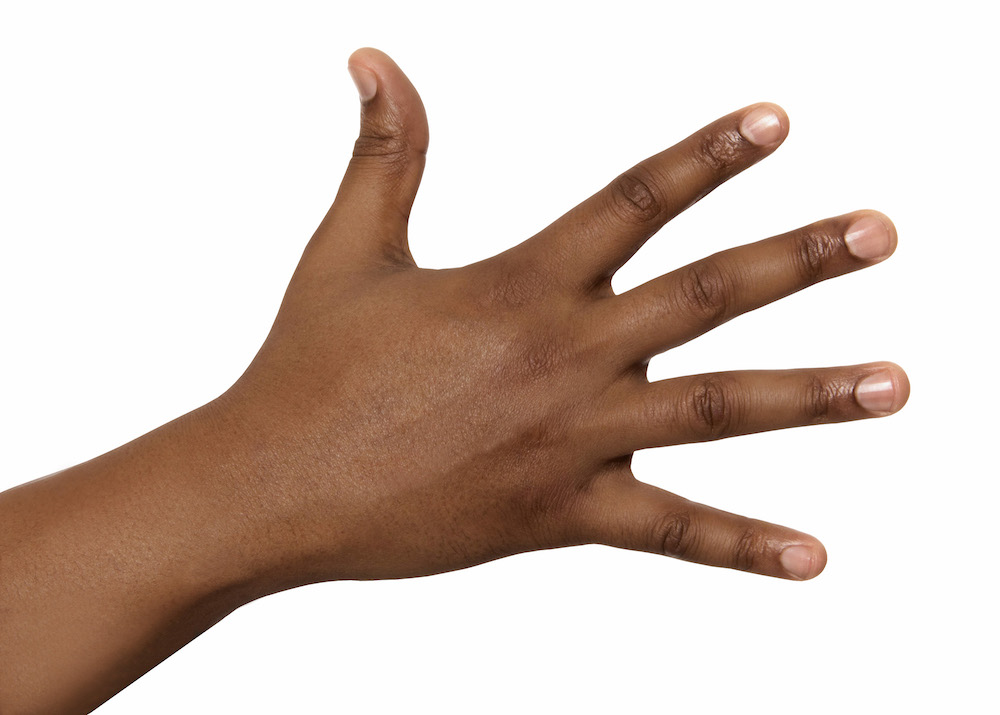
\includegraphics[width=\textwidth,height=\textheight,keepaspectratio]{../inputs/hand_dark.jpg}
  \end{minipage} & 
  \begin{minipage}{.29\textwidth}
    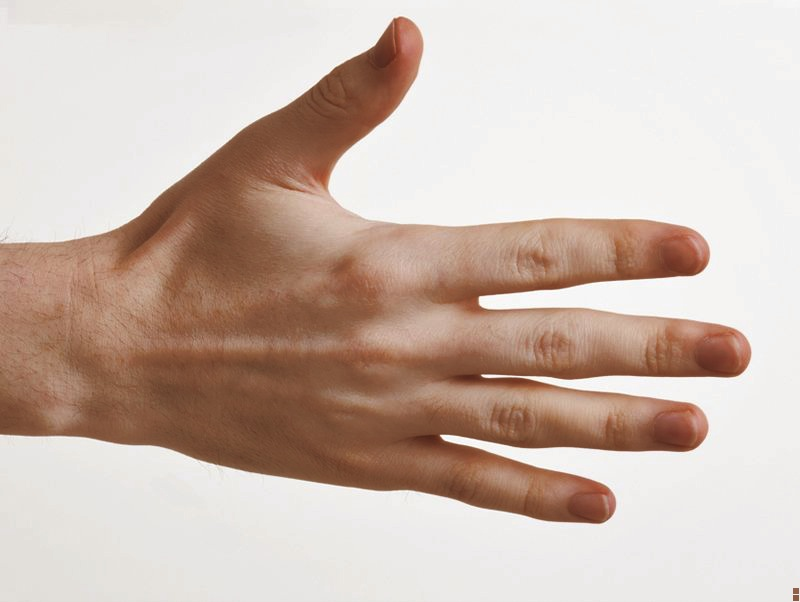
\includegraphics[width=\textwidth,height=\textheight,keepaspectratio]{../rc_test/outputs/20170522_proportional_corrected_test_alpha1p1/hand_pale_to_hand_dark.jpg}
  \end{minipage} \\
\hline  \label{row:prop_correct_test_a1p1_hand_pale_to_hand_brown} &
  \begin{minipage}{.29\textwidth}
    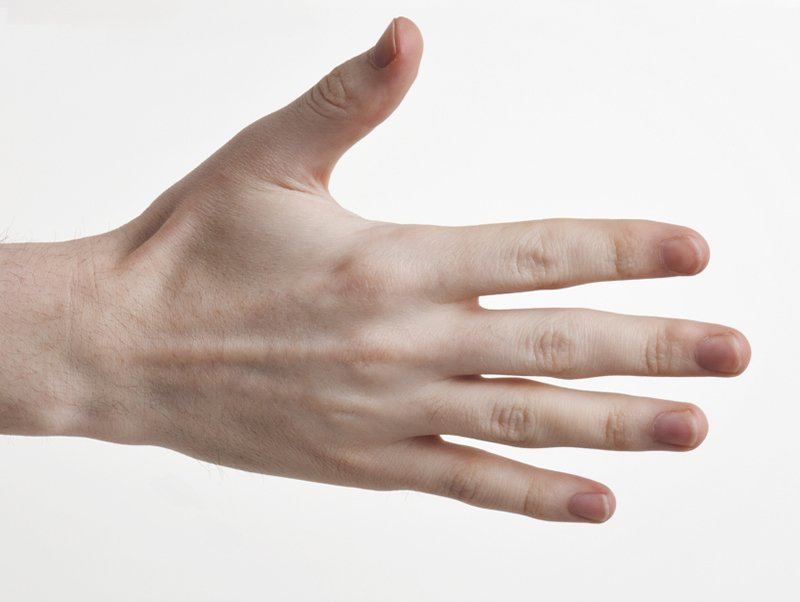
\includegraphics[width=\textwidth,height=\textheight,keepaspectratio]{../inputs/hand_pale.jpg}
  \end{minipage} & 
  \begin{minipage}{.29\textwidth}
    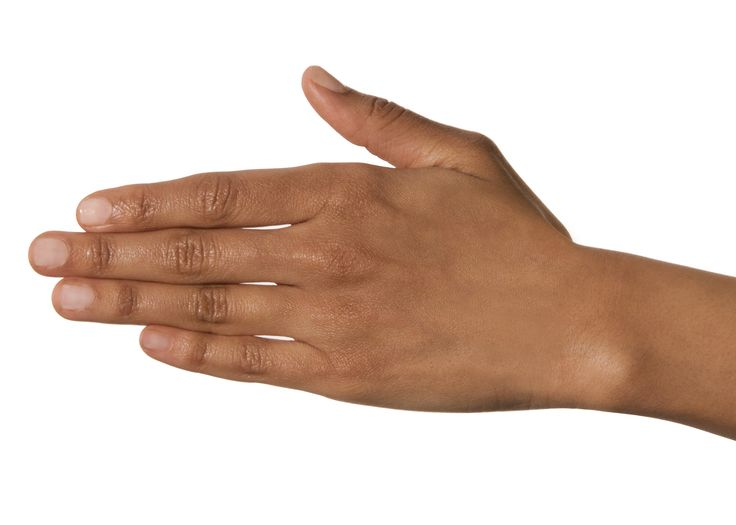
\includegraphics[width=\textwidth,height=\textheight,keepaspectratio]{../inputs/hand_brown.jpg}
  \end{minipage} & 
  \begin{minipage}{.29\textwidth}
    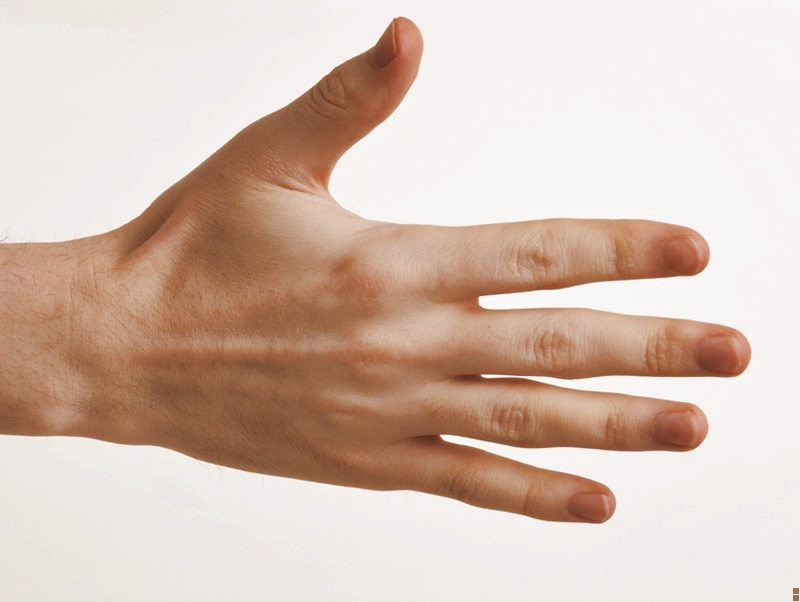
\includegraphics[width=\textwidth,height=\textheight,keepaspectratio]{../rc_test/outputs/20170522_proportional_corrected_test_alpha1p1/hand_pale_to_hand_brown.jpg}
  \end{minipage} \\
\hline  \label{row:prop_correct_test_a1p1_hand_pale_to_hand_light} &
  \begin{minipage}{.29\textwidth}
    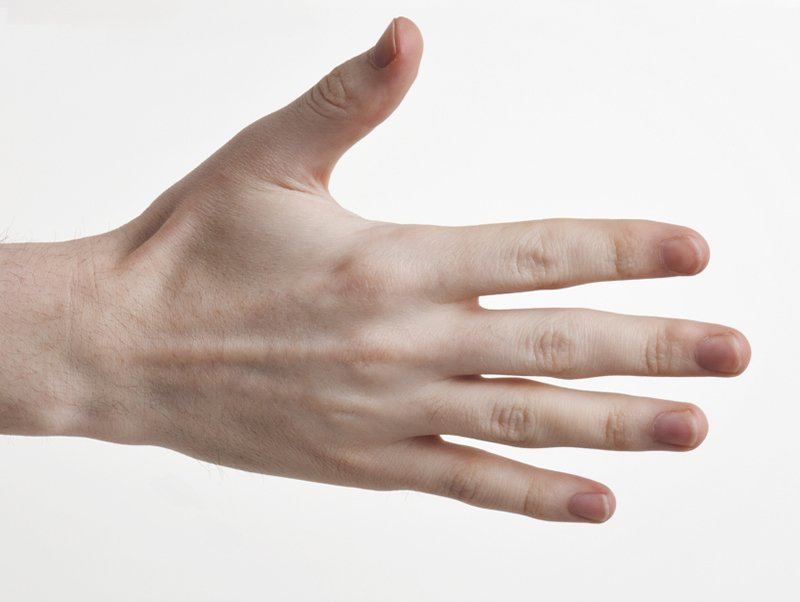
\includegraphics[width=\textwidth,height=\textheight,keepaspectratio]{../inputs/hand_pale.jpg}
  \end{minipage} & 
  \begin{minipage}{.29\textwidth}
    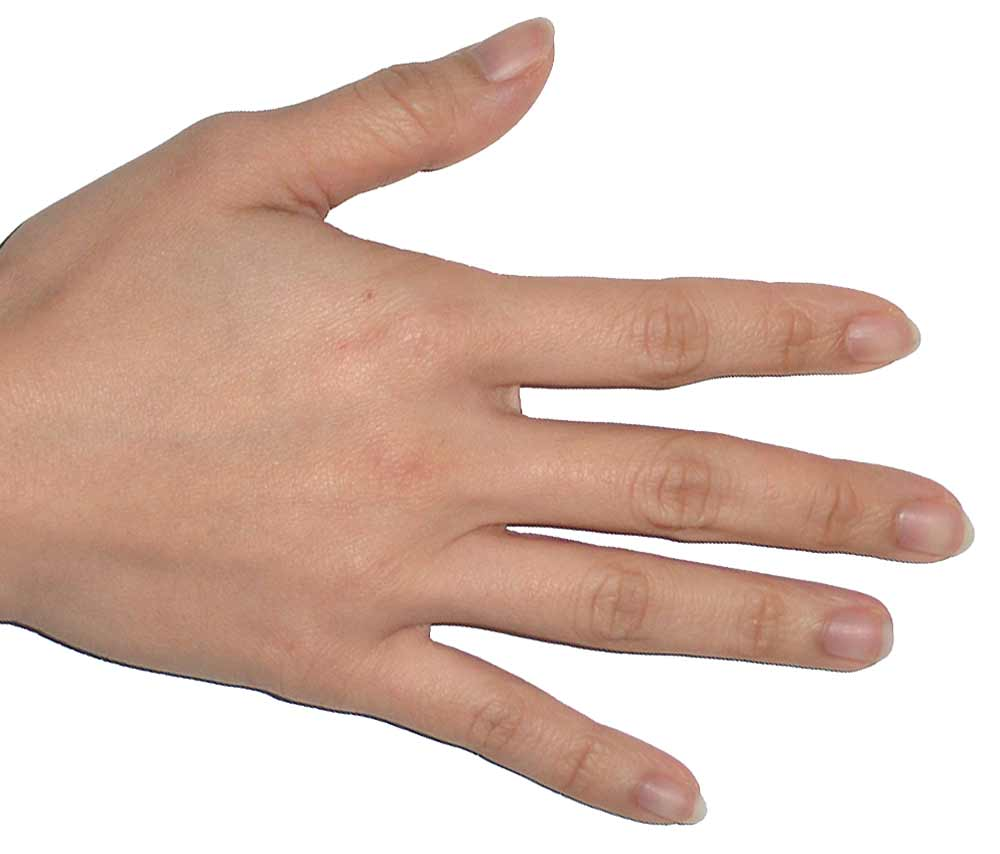
\includegraphics[width=\textwidth,height=\textheight,keepaspectratio]{../inputs/hand_light.jpg}
  \end{minipage} & 
  \begin{minipage}{.29\textwidth}
    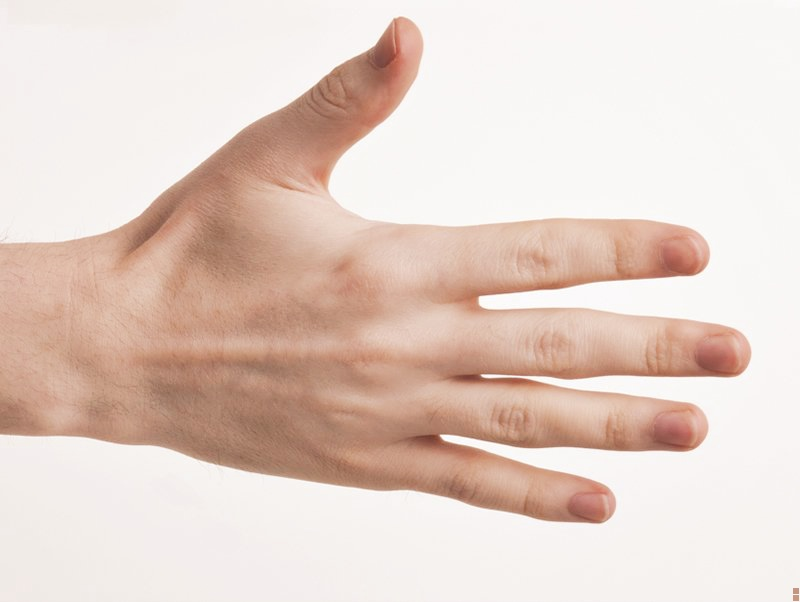
\includegraphics[width=\textwidth,height=\textheight,keepaspectratio]{../rc_test/outputs/20170522_proportional_corrected_test_alpha1p1/hand_pale_to_hand_light.jpg}
  \end{minipage} \\
\hline
 \end{longtable}

As shown in Figure \ref{img:compare_dark_spot}, the dark spots and creases noted in Section \ref{sec:algo_prop_eval} are reduced.

\begin{figure}[H]
    \centering
    \begin{subfigure}[b]{0.40\textwidth}
        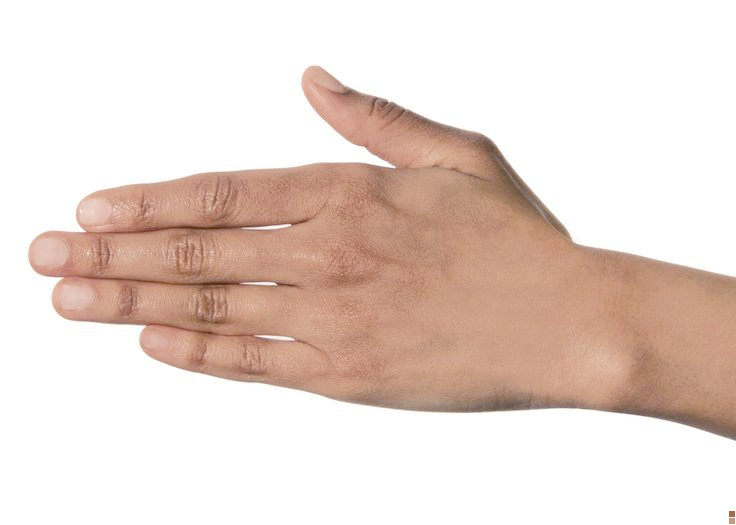
\includegraphics[width=\textwidth]{../rc_test/outputs/20170516_proportional_test/hand_brown_to_hand_light.jpg}
        \caption{Proportional adjustment algorithm (Algorithm \ref{eq:prop_algo}) result}
    \end{subfigure}
    ~
    \begin{subfigure}[b]{0.40\textwidth}
        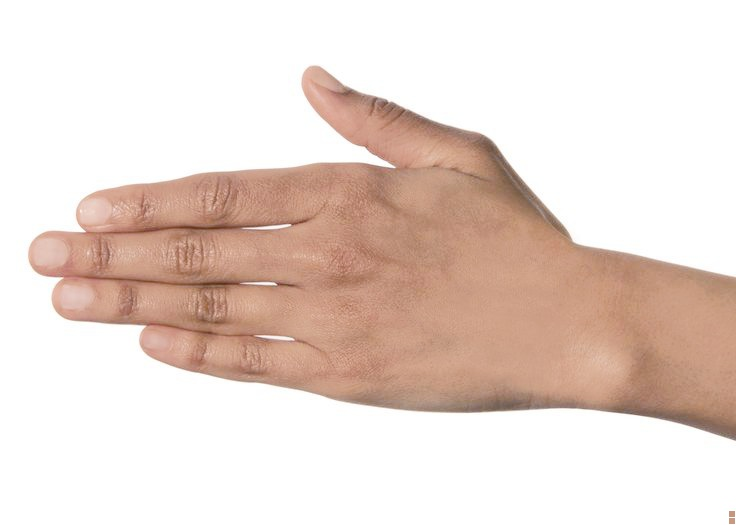
\includegraphics[width=\textwidth]{../rc_test/outputs/20170522_proportional_corrected_test_alpha1p1/hand_brown_to_hand_light.jpg}
        \caption{Proportional adjustment algorithm with correction (Algorithm \ref{eq:prop_corr_algo}) result}
    \end{subfigure}
    \caption{Comparison of Algorithms \ref{eq:prop_algo} and \ref{eq:prop_corr_algo} results for transforming a mid-toned hand (Figure \ref{img:input_hands_1_brown}) to a light hand (Figure \ref{img:input_hands_1_light}).\label{img:compare_dark_spot}}
\end{figure}

We tried this effect for a range of $\alpha$ and found that $\alpha = 1.1$ gives an acceptably realistic result. A larger $\alpha$ (such as the case for $\alpha = 5$ shown in Appendix \ref{app:prop_corr_ave_a5}) would further reduce the dark spots on the skin but may begin to strongly brighten the shadows of the image, resulting in an unrealistic effect.

Up to the current iteration the more extreme changes of colour, such as from Figure \ref{img:input_hands_1_dark} to Figure \ref{img:input_hands_1_pale} and vice versa are especially unrealistic. Part of the reason is that the shadows, most prominent in Figure \ref{img:input_hands_1_pale} is causing the calculated average colour of the entire hand to be of lower luminosity than it should be. 